
\chapter{Caso Práctico: Selección de Estructura de Datos}
\label{data_struct_sel}

A esta altura ya aprendiste sobre las estructuras de datos principales
de Perl, y has visto algunos de los algoritmos que las usan.

Este capítulo presenta un caso práctico con ejercicios que te dejan 
pensar acerca de la elección de estructuras de datos y practicar 
usándolas.

Pero primero, me gustaría discutir brevemente dos estructuras condicionales
que hemos ignorado hasta ahora y proveer nuevas posibilidades sobre las
signaturas de una subrutina.
\index{signature}

\section{El Operador Condicional Ternario}
\label{ternary operator}
\index{ternary conditional operator}

Considera el siguiente código que verifica el valor de un
número entero positivo:

\begin{verbatim}
my $result;
if $num < 10 {
    $result = "Un dígito";
} else {
    $result = "Más de un dígito";
}
say $result;
\end{verbatim}

Esto es bien simple, pero un poco largo. Esto puede escribirse
en una sola línea de código en la siguiente forma:

\begin{verbatim}
say $num < 10 ?? "Un dígito" !! "Más de un dígito";
\end{verbatim}

El operador está conformado por dos partes: {\tt ??} y {\tt !!},
los cuales separan tres expresiones (de ahí su nombre de ``operador ternario``):
\index{ternary operator}
\index{operator!ternary}
\begin{itemize}
\item La condición a ser evaluada (?`es \verb|$num| menor que 10?);
\item La expresión que define el valor si la condición es verdadera;
\item La expresión que define el valor si la condición es falsa.
\end{itemize}

Esta sentencia chequea si \verb|$num| es menor que 10 y, si esto es verdadero,
imprime ``Un dígito``; si la condición es falsa, entonces imprime ``Más de un dígito``.

Este operador no provee una funcionalidad nueva; solo ofrece una sintaxis
más concisa.

Es posible anidar varios operadores ternarios para examinar múltiples opciones
sucesivamente:
\index{ternary conditional operator, nesting}

\begin{verbatim}
say $valor < 10    ?? "Un dígito"     !! 
    $valor < 100   ?? "Dos dígitos"   !!
    $valor < 1000  ?? "Tres dígitos"  !!
                      "Más de tres dígitos";
\end{verbatim}

Esta construcción es una forma de sentencia conocida algunas
veces como una \emph{sentencia de switch} porque el lenguaje
C y muchos lenguajes derivados del mismo usan la palabra clave
{\tt switch} para describir una condicional con opciones múltiples.
\index{switch statement}

Esto es mucho más conciso y usualmente más conveniente que las condicionales
anidadas {\tt if ... después ... else}, pero la siguiente sección provee un
tipo de sentencia {\tt switch} mucho más poderosa.

\section{La Sentencia ``Switch'' {\tt given ... when}}
\label{given_when}
\index{given statement}
\index{when statement}
\index{switch statement}

Perl~6 tiene una sentencia ``switch'', escrita con las palabras claves 
{\tt given} y {\tt when}. La palabra clave {\tt given} introduce la variable
o expresión que será puesta a prueba, y cada una de las sentencia {\tt when}
especifica una condición seguida por un bloque que se ejecutará si la 
condición es verdadera. Por defecto, el proceso para cuando la primera
con la primera condición que es satisfecha.

El ejemplo más arriba podría escribirse como sigue:

\begin{verbatim}
given $value {
    when 0..9      { say "Un dígito" }
    when $_ < 99   { say "Dos dígitos" }
    when /^\d**3$/ { say "Tres dígitos" }
    default        { say "Más de tres dígitos" }
}
\end{verbatim}

La sentencia \verb|given $valor| ``topicaliza`` el argumento, i.e., 
asigna el contexto de \verb|$valor| a la variable tópico \verb|$_|
(o, más precisamente, crea un sobrenombre del mismo a través de 
la variable \verb|$_|). El argumento de {\tt given} es una variable simple
en el ejemplo más arriba, pero puede ser una expresión compleja cuya evaluación
se almacena en \verb|$_|. Cada una de las condiciones {\tt when} es
chequeada contra \verb|$_|. He escrito estas condiciones en tres formas
sintácticas diferentes para ilustrar algunas de las varias posibilidades:
\index{topical variable}
\index{alias}
\begin{itemize}
\item La primera chequea contra \verb|$_| (implícitamente) contra el
rango \verb|0..9|.
\index{range operator}
\item La segunda compara explícitamente \verb|$_| con 99.
\item La tercera usa un regex para chequear si \verb|$_| tiene
tres dígitos.
\index{regex}
\item La sentencia \verb|default| se ejecuta solo si las otras condiciones
han fallado.
\index{default statement}
\end{itemize}

Solo un mensaje será imprimido, porque el proceso de coincidencia para tan
pronto una de las condiciones ha sido satisfecha, y la cláusula \verb|default|
se ejecutará solo si las otras condiciones fallaron.

Si no hay un operador específico en la cláusula {\tt when}, entonces realizará
una coincidencia inteligente de la expresión en la la cláusula {\tt when} contra
 \verb|$_|:
\index{smart match}

\begin{verbatim}
when $foo { ... }
# equivalente a: when $foo ~~ $_ { ... }
\end{verbatim}

Nota que la palabra clave {\tt given} no hace más que topicalizar
su argumento para el resto del bloque. Las cláusulas {\tt when} son las
que hacen el trabajo pesado. De hecho, podrías usar las cláusulas {\tt when}
sin {\tt given} provisto que asignes el valor correcto a \verb|$_|, lo cual,
como podrás recordar, puede hacerse con un bloque {\tt for}:
\index{for block}

\begin{verbatim}
my $val = 7;
for $val { 
    when 0..6 { say "menos que"}
    when 7 {say "Exacto";} 
    when 8..* {say "mayor que";}
}
\end{verbatim}

\index{proceed clause}
Es posible añadir una cláusula {\tt proceed} al final de cualquier de los
bloques de código condicionales para prevenir que el proceso pare
después que el bloque de código haya sido exitoso. Por ejemplo, podrías 
escribir esto:

\begin{verbatim}
given $valor {
    when 0..9      { say "Un dígito" }
    when 10..99    { say "Dos dígitos"; proceed }
    when 42        { say "La respuesta del sentido de la vida y a todo el universo" }
    when /^\d**3$/ { say "Tres dígitos" }
    default        { say "Más de tres dígitos" }
}
\end{verbatim}

En este ejemplo, si \verb|$valor| es 42, dos mensajes se imprimirán,
"Dos dígitos" y "La respuesta del sentido de la vida y a todo el universo"
porque la cláusula {\tt proceed} en el segundo bloque de código 
evita que el proceso termine con la primera coincidencia exitosa.

Grandioso, pero hay un problema. La cláusula {\tt proceed} debería usarse
con cuidado, dado que puede fácilmente conducir a resultados inesperados.
De hecho, \emph{el código de más arriba es incorrecto}: si \verb|$valor| tiene
dos dígitos pero no es 42 (si es, digamos, 43), el bloque {\tt default} 
también se ejecutará, porque la única coincidencia exitosa tenía la cláusula
{\tt proceed}, y dirá que hay más `Más de tres dígitos'' aunque esto es
obviamente falso.

\label{proceed_ex}
Como un ejercicio, prueba el código anterior con varios valores y
intenta encontrar una manera de arreglar el error con la cláusula {\tt proceed}.

Solución: \ref{sol_proceed_ex}

\section{Subrutinas con Parámetros Nombrados y Opcionales}

% Revise this definition to make it clearer.
Las subrutinas que hemos visto hasta ahora han usado parámetros
\emph{de posición}, i.e., parámetros en los cuales la atadura (\emph{binding} en inglés) 
con los argumentos de la subrutina depende en el orden de los mismos
dentro de la lista de argumentos y en la signatura de la función. 
Usualmente esto es perfectamente normal cuando el número de argumentos
pasado a la subrutina es pequeño (digamos, tres o menos).
\index{positional parameter}
\index{parameter!positional}
\index{signature}

Cuando la signatura de la subrutina se vuelve larga, el uso de 
argumentos de posición podría volverse complicado y propenso a
errores.

\subsection{Parámetros Nombrados}
\index{named parameter}
\index{parameter!named}

Los argumentos nombrados pueden suministrarse en cualquier orden:
el nombre del parámetro está atado al argumento del mismo nombre.
Por ejemplo:

\begin{verbatim}
sub dividir (:$dividendo, :$divisor where $divisor != 0) {
     return $dividendo/$divisor;
}
say dividir(dividendo => 2048, divisor => 128);      # -> 16
# o:
say dividir(divisor => 128, dividendo => 2048);      # -> 16
\end{verbatim}

Los argumentos son suministrados en la llamada de la subrutina como una
lista de pares usando la sintaxis de constructor de pares. En la signatura,
los parámetros son extraídos en la signatura con la sintaxis de "colon-pair":
el parámetro \verb|$dividendo| está atado al valor del par cuya clave es 
``dividendo`` (2048), y \verb|$divisor| está similarmente atado a 128, 
sin importar el orden de los argumentos en la llamada de la subrutina.
\index{colon-pair syntax}
\index{pair constructor}

Estos parámetros nombrados son especialmente útiles cuando el número de
argumentos es grande. Por ejemplo, no hemos hablado de la programación
orientada a objetos todavía (ver Capítulo~\ref{objects}), pero esto es como
podríamos crear un objeto de la clase (definida por el usuario) Rectángulo:

\begin{verbatim}
my $rect = Rectángulo.new( 
    origen_x  => 100, 
    origen_y  => 200, 
    ancho     => 23,
    longitud  => 42,
    color     => 'negro'
);
\end{verbatim}

Claramente, el uso de cinco parámetros de posición no sería práctico.

\subsection{Parámetros Opcionales}
\index{optional parameter}
\index{parameter!optional}
\index{variadic subroutine}
\index{signature}

Algunas veces, el número actual de argumentos no se conoce
con antelación: por ejemplo, una subrutina puede llamarse con 
un número variable de argumentos. Tal subrutina se conoce como
\emph{variádica}. Puedes definir un parámetro para que sea opcional
al colocar un signo de interrogación en frente del mismo en la
signatura de la subrutina:

\begin{verbatim}
sub my-sub($x, $y?) {  # simple parámetro opcional
    if $y.defined {
        say "El segundo parámetro ha sido suministrado y definido";
    } else {
        say "El segundo parámetro no ha sido suministrado";
    }
    # ...
}
\end{verbatim}

\index{positional parameter}
\index{parameter!positional}
Al usar parámetros de posición, los parámetros opcionales siempre
tienen que ser los últimos en la lista (después de aquellos que 
son argumentos).

Un parámetro puede también hacerse opcional al suministra un:
{\bf valor por defecto}:
\index{default value}
\index{default parameter}
\index{parameter!default value}

\begin{verbatim}
sub mi-log($número, $base = e) {    # e es una constante predefinida
                                    # $base es un parámetro opcional
    return log($número) / log($base);
}
say mi-log(4);       # Logaritmo natural (base e)  -> 1.38629436111989
say mi-log(32, 2);   # Logaritmo en base 2         -> 5
say mi-log(100, 10); # Logaritmo común (base 10)   -> 2
\end{verbatim}

Aquí, si el segundo argumento no se suministra, el valor por defecto 
(\emph{e}) es usado. Inversamente, si hay un segundo argumento, este
{\bf anula} el valor por defecto.

\index{slurpy parameters}
\index{parameter!slurpy}
\label{slurpy_parameters}
En algunas ocasiones, tener parámetros opcionales o por defecto no
es suficiente. Por ejemplo, la subrutina puede tener que procesar una 
lista que contiene un número indeterminado de valores. Para situaciones
como esta, puedes usar un \emph{parámetro slurpy}, i.e., un tipo de
array colocado al final de la lista de parámetros que consumirá todos los 
argumentos restantes. Este tipo de parámetro slurpy usa el sigilo \verb|*@|.
En el ejemplo siguiente, la subrutina toma un parámetro mandatario
(el primer número de la lista) y un lista de argumentos adicionales
que serán almacenados en el array \verb|@resto|:
\index{twigil}

\begin{verbatim}
sub mi-suma($primer-num, *@resto) {
    say @resto;                      # -> [3 4 5 12 17]
    return $primer-num + [+] @resto;
}
say mi-suma 1, 3, 4, 5, 12, 17;      # -> 42 
\end{verbatim}

Otros ejemplos de los parámetros slurpy se han proveído
en la Sección~\ref{sol_exercise_queue}.

\section{Análisis de la Frecuencia de Palabras}
\label{analysis}

Ahora, hablemos del caso práctico.

Como es habitual, deberías por lo menos intentar los
ejercicios antes de leer las soluciones sugeridas, las cuales
se proveen en las secciones siguientes de este capítulo.

\begin{exercise}

Escribe un programa que lee un archivo, descompone cada línea en palabras,
remueve los espacios en blanco y signos de puntuación de la palabra,
y las convierte a palabras minúsculas.

\end{exercise}


\begin{exercise}
\index{Project Gutenberg}

Dirígete a Project Gutenberg (\url{http://gutenberg.org}) y descarga tu 
copia de libro favorito en formato de texto simple.
\index{plain text}
\index{text!plain}

Modifica tu programa del ejercicio previo para que lea el libro que descargaste,
salta sobre la información de la cabecera al principio del archivo, y procesa el 
resto de las palabras como lo hiciste anteriormente.

Después modifica el programa para que cuente el número total de palabras en
el libro, y el número de veces que cada palabra es usada.
\index{word frequency}
\index{frequency!word}

Imprime el número de palabras diferentes usadas en el libro. Compara
libros diferentes por autores diferentes, escritos en eras diferentes. 
?`Cuáles autores usan el vocabulario más extenso?
\end{exercise}


\begin{exercise}

Modifica el programa del ejercicio anterior para que imprima las
20 palabras más frecuentemente usadas en un libro dado,

\end{exercise}


\begin{exercise}

Modifica el programa anterior para que lea una lista de palabras (ver Sección~\ref{wordlist})
y después imprima todas las palabras en el libro que no están en la 
lista de palabras. ?`Cuántas de ellas son errores tipográficos? ?`Cuántas de ellas
son palabras comunes que {\emph deberían} estar en la lista de palabras, y cuántas de
ellas son realmente recónditas?

\end{exercise}


\section{Números Aleatorios}
\index{random number}
\index{number, random}
\index{deterministic}
\index{pseudorandom}

Dada la misma entrada, la mayoría de programas de computadoras generan
la misma salida cada vez y, por lo tanto, se dice que son {\bf deterministas}.
El determinismo es usualmente algo bueno, dado que esperamos que 
la misma computación produzca el mismo resultado. Aunque, para algunas aplicaciones,
queremos que la computadora sea impredecible. Los juegos de computadora
son un ejemplo obvio, pero existen más.

Hacer un programa verdaderamente no determinista resulta ser algo difícil,
pero hay algunas manera de hacerlo parecer por lo menos no determinista. 
Una de ellas es usar algoritmos que generan números {\bf pseudoaleatorios}.
Los números pseudoaleatorios no son verdaderamente aleatorios porque son
generados a través de una computación determinista, pero solo con mirarlos
es imposible distinguirlos de los números aleatorios.

Perl provee funciones tales como {\tt rand} que generan números pseudoaleatorios
(los cuales llamaremos simplemente números ``aleatorios`` de aquí en adelante).
\index{rand function}
\index{function!rand}

La función {\tt rand} devuelve un número aleatorio (del tipo {\tt Num}) entre
0.0 y 1.0 (incluyendo a 0.0 pero no a 1.0). Cada vez que llamas a {\tt rand},
obtienes el número siguiente en una serie larga. Para ver una muestra, ejecuta
este bucle en el REPL:

\begin{verbatim}
say rand for 1..5;
\end{verbatim}

Cuando se usa como un método, {\tt rand} devuelve un número aleatorio entre
0.0 y el valor del invocante. Por ejemplo, {\tt 10.rand} devuelve un número
aleatorio entre 0 y 10 (excluyendo al 10). Podrías intentarlo como un programa
de una sola línea:
\index{one-liner mode}

\begin{verbatim}
$ perl6 -e 'say 10.rand for 1..5'
8.23987158729588
9.83276889381497
2.52313276833335
3.44713459548771
1.82329894347025
\end{verbatim}

Con suerte, deberías obtener una salida diferente a la que obtuve.
Si quieres ejecutar un programa de una sola línea en Windows,
recuerda que necesitarás reemplazar las comillas simples con comillas
dobles.

Para obtener números enteros aleatorios entre 1 y 10, podrías usar 
los métodos {\tt Int} y {\tt rand}:
\index{Int function or method}

\begin{verbatim}
$ perl6 -e 'say 10.rand.Int + 1 for 1..5'
5
10
1
6
3
\end{verbatim}

La función o método {\tt pick} toma un número \verb|$n| y una lista 
como argumentos y devuelve \verb|$n| artículos escogidos aleatoriamente
y sin repetición. Por ejemplo:
\index{pick function or method}

\begin{verbatim}
> say <1 3 4 5 7 9 10 12 14 42>.pick(5);
(5 42 3 4 7)
> say pick 5, <1 3 4 5 7 9 10 12 14 42>;
(42 12 5 1 9)
\end{verbatim}

Si \verb|$n| es mayor o igual al número de artículos de la lista,
entonces todos los elementos de la lista será devueltos en una
secuencia aleatoria.

Para obtener enteros aleatorios únicos en un rango, podrías usar
{\tt pick} en un rango:

\begin{verbatim}
> say pick 5, 1..20;
(5 3 6 18 7)
> say (1..20).pick(5);
(20 4 18 2 7)
\end{verbatim}

Si no especifica la cantidad de números aleatorios, obtendrás un
solo número aleatorio:

\begin{verbatim}
> say (1..20).pick;
19
\end{verbatim}
%


\begin{exercise}
\index{histogram!random choice}

Escribe una función nombrada \verb"escoge_del_hist" que toma un
histograma como definido en la Sección~\ref{histogram} y devuelve 
un valor aleatorio del histograma, elegido con una probabilidad 
proporcional a la frecuencia. Por ejemplo, para tres artículos:
\verb|('a', 'a', 'b')|, tu función debería devolver \verb|a| con una
probabilidad de $2/3$ y \verb|'b'| con una probabilidad de $1/3$.
\end{exercise}


\section{Histograma de Palabras}

Deberías intentar solucionar el ejercicio anterior antes
de proceder.

Para el propósito de presentar las soluciones a los ejercicios anteriores,
he usado el texto sencillo de {\em Don Quijote} (1605 y 1615), una novela escrita
por Miguel de Servantes, descargada desde el proyecto Gutenberg
(\url{https://www.gutenberg.org/files/2000/2000-8.txt}) y guardada en
un archivo llamado \emph{quijote.txt}
\footnote{Si tienes algún problema
con el archivo, puede deberse a cambios hecho al formato del mismo por
el proyecto Gutenberg. Para evitar tal problema asociado con cualquier
cambio (y otros cambios futuros), puedes descarga el archivo original
desde este repositorio de Gitlab: \url{https://gitlab.com/uzluisf/piensaperl6/tree/master/suplementos/quijote.txt}}.
Usa el mismo texto si quieres comparar tus soluciones y los resultados con los míos.

% https://github.com/LaurentRosenfeld/thinkperl6/blob/master/Supplementary/emma.txt
\index{de Servantes, Miguel}
\index{Don Quijote}
\index{Project Gutenberg}

\begin{description}
\item {\bf Nota del traductor}:	En {\em Think Perl 6}, el autor usa el texto de la novela
\emph{Emma}, escrita por Jane Austen\footnote{Puedes encontrar el archivo en este repositorio: 
\url{https://github.com/LaurentRosenfeld/thinkperl6/blob/master/Supplementary/emma.txt}.
De igual manera, puedes consultar Think Perl 6 para comparar tus resultados con los del 
autor si decides usar este texto.}. He decidido usar un libro en español porque creo que es más ameno y porque quería saber cuantas palabras tenía el libro \emph{Don Quijote de la Mancha}.
\end{description}

Aquí esta el programa que lee el archivo \emph{quijote.txt} y construye un
histograma de las palabras  en el archivo que pertenecen al libro:
\index{histogram!word frequencies}

\begin{verbatim}
my %histograma;
my $saltar = True; # bandera para saltar la cabecera y 
                   # marcar el final del libro

sub procesar-línea(Str $línea is copy) {
	if defined index $línea, "*** START OF THIS PROJECT" {
		$saltar = False ;
		return;
	}

	return if $línea ~~ / Abela || anonymous /; 
	return if $saltar;
	$línea ~~ s:g/<['-]>/ /;             # Reemplazar guiones y apóstrofos con espacios
	$línea ~~ s:g/<[;:,¡!¿?«».()"_`]>//; # Remover signos de puntuación
	$línea = $línea.lc;                  # Convertir cadena a minúscula
	for $línea.words -> $palabra {
		%histograma{$palabra}++;
	}

	$saltar = True if $línea ~~ /^fin$/; # Marcar el final del libro
}
procesar-línea $_ for "quijote.txt".IO.lines; 
\end{verbatim}

\index{case!lower}
%

El programa lee cada línea del archivo \emph{quijote.txt} file y,
por cada línea, llama a la subrutina \verb|procesar-línea|.

\index{accumulator!histogram}
La subrutina \verb|procesar-línea| salta las líneas de la cabecera
(i.e., todas las líneas hasta que se encuentra la línea que contenga
la cadena de texto ``*** START OF THIS PROJECT``). De igual manera,
también salta cualquier línea que contenga las palabras ``Abela`` o
``anonymous``. La función reemplaza 
los guiones y los apóstrofos con espacios en blanco, remueve varios 
caracteres de puntuación, y convierte la línea a minúscula. Después,
divide la línea en palabras individuales que son almacenadas y 
contadas con un acumulador en el hash \verb|%histograma|.  Al final
asigna verdadero a \verb|$saltar| si la línea contiene solo la 
palabra ``fin``, la cual marca el final del texto.

Para saber si el programa está haciendo lo que esperamos que haga,
podemos mostrar unas entradas del hash \verb|%histograma|:

\begin{verbatim}
# mostrando 20 líneas del histograma
my $cuenta;
for %histograma -> $par {
say sprintf "%-24s %d", $par.key, $par.value;
$cuenta++;
last if $cuenta > 20;

}
\end{verbatim}

Esto imprime lo siguiente:

\begin{verbatim}
ahorcase                 1
descontente              1
regüeldos                1
libras                   5
manteca                  1
suerte                   141
voy                      51
desnudaba                1
xxviii                   2
benevolencia             2
vieren                   3
rebenque                 1
asentado                 2
profetizadas             2
mirábalas                1
lata                     4
cesaría                  1
preguntalle              1
bailado                  2
elogio                   2
codicio                  1
\end{verbatim}

Para contar el número total de palabras (pertenecientes al libro) en el archivo,
podemos añadir los valores en el histograma:

\begin{verbatim}
my $total_palabras = [+] %histograma.values;
say "Hay $total_palabras palabras en el libro.";
\end{verbatim}
%
El número de palabras diferentes es solo el número de artículos en
el hash:

\begin{verbatim}
my $palabras-distintas = %histograma.elems;
say "Hay $palabras-distintas palabras distintas en el libro.";
\end{verbatim}
%
Nota que podrías reducir lo anterior a una línea de código al
interpolar un bloque de código dentro de la cadena de texto de salida:
\index{interpolating a code block in a string}

\begin{verbatim}
say "Hay {%histograma.elems} palabras distintas en el libro.";
\end{verbatim}
%
Y los resultados:

\begin{verbatim}
Hay 381215 palabras en el libro.
Hay 22950 palabras distintas en el libro.
\end{verbatim}
%


\section{Palabras Más Comunes}
\label{most_common_words}

Para encontrar las palabras más comunes en \verb|quijote.txt|,
podemos ordenar el hash \verb|%histograma| de acuerdo a los 
valores (frecuencia de palabras) y extraer las 10 palabras más
frecuentes en un array.
\index{sort}

\begin{verbatim}
my @más_comunes = (sort { %histograma{$^b} cmp %histograma{$^a} }, 
                    %histograma.keys)[0..9];
say $_ for map { "$_ \t%histograma{$_} "}, @más_comunes;
\end{verbatim}

Las funciones {\tt sort} recibe las claves del histograma y su función 
de comparación compara los valores asociados con esas claves. Dado que
usamos la clave \verb|$^b| antes que la clave \verb|$^a|, {\tt sort}
producirá un ordenamiento en orden reverso (descendente). El procedimiento
{\tt sort} completo está colocado dentro de paréntesis, para que el rango 
de subíndices {\tt [0..9]} actúe como una rebanada sobre la lista producida por
{\tt sort} y retiene solo las primeras 10 palabras más frecuentes. El resultado
se almacena en el array \verb|@más_comunes|. La siguiente línea de código 
solo procesa el array para mostrar las palabras y sus frecuencias respectivas.
\index{slice}

Esto muestra la siguiente salida:

\begin{verbatim}
que     20626 
de      18214 
y       18188 
la      10363 
a       9823 
en      8241 
el      8210 
no      6335 
los     4748 
se      4690 
\end{verbatim}
%
Si quieres ver más palabras interesantes, podrías, como un ejercicio
adicional, filtrar el histograma y retener solo las palabras
que tienen más de, digamos, cuatros letras.

El array temporario \verb|@más_comunes| no es realmente necesario.
Podríamos hacer todo el proceso con una sola sentencia:

\begin{verbatim}
say $_ for map { "$_ \t%histograma{$_} "},  
           (sort { %histograma{$^b} cmp %histograma{$^a} }, 
           %histograma.keys)[0..9];
\end{verbatim}

Este es un ejemplo de la programación de tuberías. Este tipo de sentencia
necesita leerse de abajo hacia arriba y de derecha a izquierda. El 
primer paso es \verb|%histograma.keys|, el cual produce una lista de
las claves del histograma; esta lista se suministra a la sentencia {\tt sort}
para producir una lista de las llaves ordenadas (en orden descendente)
de acuerdo a sus valores; una vez que esta parte entre los paréntesis
se ha completado, el rango de subíndices \verb|[0..9]| retiene las 10 
palabras más frecuentes y las administra a la sentencia map, la cual 
produce la lista de palabras y las frecuencias para la salida final.

Déjame agregar una palabra de advertencia: ordenar el histograma
por los valores y escoger los 10 más frecuentes para obtener las
palabras más frecuentes es probablemente la manera más fácil de 
resolver el problema y el código más corto para hacerlo.
Esta es la razón por la cual he usado esta solución aquí. Pero no es la
solución más eficiente desde el punto de vista del tiempo de ejecución,
porque involucra el costo de ordenar un conjunto de datos relativamente
grade, donde solo usamos una parte pequeña de los datos ordenados. Hay
algoritmos mejores para hacer eso desde el punto de vista de la
eficiencia de ejecución, pero son más complicados. Por lo tanto, hay 
un sacrificio entre la eficiencia de código y el rendimiento. Asumiendo que 
esto es código que queremos ejecutar solamente una vez, he favorecido
la eficiencia de código.
\index{data pipeline programming}


\section{Parámetros Opcionales}
\index{optional parameter}
\index{parameter!optional}

Vimos anteriormente en este capítulo que las subrutinas pueden tomar
parámetros opcionales. Podemos usar esta funcionalidad para escribir
una subrutina que imprime las palabras más comunes en el 
hash \verb|%histograma| extraído desde \emph{quijote.txt}.

\begin{verbatim}
mostrar-más-comunes(%histograma, 5);

sub mostrar-más-comunes( %hist, Int $num = 10 ) {
    say $_ for map { "$_ \t%hist{$_} "}, 
    (sort { %hist{$^b} cmp %hist{$^a} },
    %hist.keys)[0..$num - 1];
}
\end{verbatim}

Esto mostrará las 5 palabras más comunes de la lista más
arriba (Sección~\ref{most_common_words}). Si la llamamos
sin el segundo parámetro:

\begin{verbatim}
mostrar-más-comunes(%histograma);
\end{verbatim}

obtendremos las 10 palabras más comunes (misma lista como la
que mostramos en la Sección~\ref{most_common_words}), porque el 
valor por defecto para el segundo parámetro es 10.

\section{Diferencia de Hashes}
\label{hashsub}
\index{hash!subtraction}
\index{subtraction!hash}

Encontrar las palabras en \emph{quijote.txt} que no están en la lista
de palabras {\tt lemario.txt} es un problema que podrías reconocer como una 
diferencia de conjuntos; es decir, queremos encontrar todas las palabras
en un conjunto (las palabras en \emph{quijote.txt}) que no están en el
otro (las palabras en \emph{lemario.txt}).

La subrutina {\tt sustraer} toma los hashes \verb|%princ| y \verb|%dicc|
y devuelve un nuevo hash que contiene todos las claves de \verb|%princ|
que no están en \verb|%dicc|. Dado que no nos importan los valores, asignamos
1 a todas la claves.

\begin{verbatim}
sub sustraer (%princ, %dicc) {
	my %diferencia;
	for %princ.keys -> $palabra {
		%diferencia{$palabra} = 1 unless %dicc{$palabra}:exists;
	}
	return %diferencia;
}
\end{verbatim}
%
Para encontrar las palabras en \emph{quijote.txt} que no están en 
\emph{lemario.txt}, necesitamos carga la lista de palabras en un hash
y llamar a {\tt sustraer}, pasando los dos hashes como argumentos. 
También agregamos algunas líneas código para imprimir las primeras 20 palabras 
que no se encuentran en la lista de palabras:

\begin{verbatim}
my %lista-palabras = map { $_ => 1 }, "lemario.txt".IO.lines;
my %palabras-desconocidas = subtract(%histograma, %lista-palabras);
say %palabras-desconocidas.keys.head(20);
\end{verbatim}
%
\index{head}
Nota que en lugar de usar una rebanada, he usado el método {\tt head}
para imprimir las primeras 20 palabras de la lista. Esta es solo otra
manera de obtener los primeros ``n`` artículos de una lista o un
array. También existe un método {|tt tail} que extrae los últimos
``n`` artículos de una lista o un array.
\index{head method}
\index{tail method}

Aquí están algunos de los resultados de {\em Don Quijote}:

\begin{verbatim}
(ahorcase descontente regüeldos manteca suerte voy desnudaba 
xxviii benevolencia vieren rebenque asentado profetizadas 
mirábalas lata cesaría preguntalle bailado elogio codicio)
\end{verbatim}
%
Algunas de estas palabras son nombres y números romanos. Otras
son raras y posiblemente no en uso. Otras son verbos conjugados.
!`Pero algunas son palabras comunes que deberían  estar en la lista!

Nota que aquí he usado un hash (\verb|%palabras-desconocidas|) para almacenar las 
palabras de \emph{quijote.txt} que no se encuentran en la lista de palabras.
Dado que estamos utilizando los datos solo para imprimir una muestra de 20 palabras,
podríamos haber usado un array.

\section{Construir Operadores Nuevos}

\label{operator_construction}
\index{hash!subtraction}
\index{creating new operators}
\index{new operators!creating}
\index{overload operators}
\index{operator!overloading}
\index{operator construction}

Aprender sobre la diferencia de sustracción es una oportunidad
excelente de introducir una funcionalidad muy interesante de Perl~6:
la capacidad de construir operadores nuevos o redefinir aquellos existentes.

Dado que estamos sustrayendo dos listas de palabras, es muy tentador usar
el signo de menos para denotar esta operación de sustracción. Es muy fácil 
crear tal operador en Perl~6:

\begin{verbatim}
multi sub infix:<-> (%princ, %dicc) {
	my %diferencia;
	for %princ.keys -> $palabra {
		%diferencia{$palabra} = 1 unless %dicc{$palabra}:exists;
	}
	return %diferencia;
}
\end{verbatim}

\index{infix}
\index{subroutine signature}
\index{signature}
\index{multi!subroutine}

Comparada con la definición de la subrutina {\tt sustraer}, la
única diferencia se encuentra en la línea cabecera. Discutiremos
los detalles en un capítulo más adelante, pero los explicaremos
brevemente aquí. La mayoría de los operadores de Perl~6 son definidos
como subrutinas ``multis``, i.e., subrutinas que pueden ser definidas
varias veces con diferentes signaturas y cuerpos; Perl sabrá cual debe usar
dependiendo en la signatura. Aquí definimos el operador de menos como
una subrutina multi cuyos parámetros son dos hashes; esto será 
suficiente para que el compilador de Perl sepa que no queremos usar
la sustracción regular entre dos valores numéricos, pero algo más que
aplica a dos hashes. El operador de menos está definido como como un ``infijo``,
lo cual significa que el operador será colocado entre sus dos
operadores.

Llamar este operador es tan fácil como llamar el operador regular de 
sustracción entre dos números; solo necesitamos usar dos hashes como
operandos:

\begin{verbatim}
my %palabras-desconocidas = %histograma - %lista-palabras;
\end{verbatim}

El resto del programa funciona como antes.

\index{extending the language}
Esta facilidad para crear operadores nuevos es una de las facilidades
ofrecidas por Perl~6 parae \emph{extender el lenguaje} desde si mismo.
Regresaremos a eso y otras maneras de extender el lenguaje en los
capítulos siguientes.

\label{fact_operator}
\index{factorial}
\index{factorial!operator}
Como un ejercicio, escribe una subrutina multi que crea un nuevo operador
``!`` para calcular el factorial de un entero:
\index{factorial}

\begin{verbatim}
say 5!;     # -> 120
\end{verbatim}
%
También intenta pensar cómo probarías este nuevo operador ``!``
con varios valores de entrada.
Solution: \ref{sol_fact_operator}


\section{Sets, Bags y Mixes}
\label{sets_and_bags}

\index{set}
\index{type!set}
\index{bag}
\index{type!bag}
\index{mix}
\index{type!mix}
\index{sethash}
\index{type!sethash}
\index{baghash}
\index{type!baghash}
\index{mixhash}
\index{type!mixhash}

Perl~6 tiene una variedad de tipos de estructuras de datos llamadas
{\tt Set}, {\tt Bag} y {\tt Mix} que proveen muchas operaciones de
conjuntos comunes. Estas estructuras son colecciones desordenadas de
artículos {and weighed} únicos. Ellas son inmutables (pero también hay
versiones mutables de estas estructuras de datos, {\tt SetHash}, {\tt BagHash} 
y {\tt MixHash}).

Puedes crear y usar un conjunto en la siguiente forma:

\begin{verbatim}
> my $s = set <banana manzana naranja naranja banana pera manzana>;
set(banana, naranja, manzana, pera)
> say $s.perl
set("banana","naranja","manzana","pera")
> say $s.elems;
4
> say $s{'manzana'}
True
> say $s{'cereza'}
False
\end{verbatim}
%
Como puedes ver, los duplicados han sido removidos. Los conjuntos
solo nos dicen si al menos un elemento de un nombre dado se ha visto. 

Un bag, al contrario, también mantiene un registro del número de
cada artículo que se ha visto:

\begin{verbatim}
> my $b = bag <banana manzana naranja naranja banana pera manzana>;
Bag(banana(2), naranja(3), pera, manzana(2))
> say $b{'banana'}
2
\end{verbatim} 

Los mixes son similares a los bags, excepto que el peso de los elementos
no tiene que ser entero.

La cosa interesante acerca de estas colecciones es que pueden usar
muchas de las operaciones comunes de conjuntos usadas en matemáticas,
tales como el operador de membresía de conjunto \verb|∈| (o usa \verb|(elem)|
si no sabes como teclearlo \verb|∈| en tu editor~\footnote{No puedo
enseñarte como teclear estos caracteres, porque cada editor requiere
métodos diferentes.}), el operador de intersección de conjunto \verb|∩| o
\verb|(&)|, y el operador de subconjunto \verb'⊂' o \verb'(<)':

\begin{verbatim}
> say "Encontrado!" if 'manzana' (elem) $s;
Encontrado!
> say "Es un subconjunto!" if <naranja banana> (<) $s;
Es un subconjunto!
> say <naranja banana piña> (&) $s;
set(banana, naranja)
\end{verbatim}

Nota que no hemos usado la palabra clave {\tt set} para definir
la lista \verb|<naranja banana>| en el segundo ejemplo más arriba.
Esta lista ha sido coaccionado en un {\tt Set} para chequear si era
un subconjunto del conjunto \verb|$s|. Esta es una de las cosas 
grandiosas de estas colecciones: la mayoría de estos operadores de
conjuntos pueden usarse con listas, arrays, y hashes.
\index{coercion}

\index{set!membership operator}
\index{operator!set membership}
Podemos escribir el programa de la diferencia de hashes usando
un conjunto para la lista de palabras y el operador de membresía
de conjunto  \verb|∈| (o \verb|(elem)|):

\begin{verbatim}
my %histograma;
my $saltar = True; # bandera para saltar la cabecera
sub procesar-línea(Str $línea is copy) {
    # (igual que antes)
}

procesar-línea $_ for "lemario.txt".IO.lines; 
my $lista-palabras = set "lemario.txt".IO.lines;
my %palabras-desconocidas = sustraer(%histograma, $lista-palabras);
say %palabras-desconocidas.keys.head(20);

sub sustraer (%princ, $dicc) {
    my %diferencia;
    for %princ.keys -> $palabra {
        %diferencia{$palabra} = 1 unless $palabra (elem) $dicc;
    }
    return %diferencia;
}
\end{verbatim}

La línea de código en el bucle {\tt for} podría también
escribirse como sigue:
\index{set!contain operator}
\index{operator!set contain}
\begin{verbatim}
       %diferencia{$palabra} = 1 unless $palabra ∈ $dicc;
#o:    %diferencia{$palabra} = 1 if $palabra ∉ $dicc;
#o:    %diferencia{$palabra} = 1 if $palabra !(elem) $dicc;

#o hasta con el operador (cont) o ∋:
       %diferencia{$palabra} = 1 unless $dicc (cont) $palabra;
#o:    %diferencia{$palabra} = 1 unless $dicc ∋ $palabra;
#o:    %diferencia{$palabra} = 1 if $dicc ∌ $palabra;
# etc.
\end{verbatim}

\index{set!difference operator}
\index{operator!set difference}
Los operadores integrados \verb|∖| \footnote{Ten presente que 
este es el carácter unicode {\tt 2216}, no la misma barra
invertida $\backslash$} y \verb|(-)| proveen la diferencia de
conjunto, así que no tenemos ni que escribir una subrutina {\tt sustraer}
ni construir nuestro propio operador de menos:

\begin{verbatim}
procesar-línea $_ for "quijote.txt".IO.lines; 
my $lista-palabras = set "lemario.txt".IO.lines;
my $palabras-desconocidas = %histograma.keys (-) $lista-palabras;
say $palabras-desconocidas.keys.head(20);
\end{verbatim}

Hay más de 30 operadores de conjuntos disponibles, que cubren la
mayoría de los operadores de conjuntos usados en matemática. 
Solo he mostrado aquellos que pueden ser más útiles. Chequea
la documentación oficial (\url{https://doc.perl6.org/language/setbagmix}) 
si necesitas otros operadores.

\label{diff_with_set}
Como un ejercicio, puedes escribir la subrutina {\tt procesar-línea}
de nuevo o reemplazarla para usar un set o un bag en lugar de un hash
para almacenar las palabras de \emph{quijote.txt} (y posiblemente adaptar
el resto del programa donde sea necesario), para encontrar las palabras
de \emph{quijote.txt} que no se encuentran en \emph{lemario.txt}
Solución: \ref{sol_diff_with_set}


\section{Palabras Aleatorias}
\label{randomwords}
\index{histogram!random choice}

Para elegir palabras aleatorias desde el histograma, el algoritmo más
simple es construir una lista con copias múltiples de cada palabra,
de acuerdo a la frecuencia observada, y después escoges desde la
lista con la función \verb|pick|:
\index{pick function or method}

\begin{verbatim}
my @array = map {| (.key xx .value)}, %histograma;
say pick 30, @array;
\end{verbatim}
%
La expresión \verb'map {| (.key xx .value)}' lee cada par del
histograma y crea una lista con copias {\tt .value} de la cadena
en {\tt .key}. La función {\tt pick} selecciona 30 palabras aleatorias
desde el array.

Este algoritmo funciona, pero no es muy eficiente; cada vez que eliges
un o más palabras aleatorias, se reconstruye la lista, la cual es tan
grande como el libro original. Una mejora obvia es construir la lista una
sola vez y después hacer selecciones múltiples, pero la lista es aún
grande.

Una alternativa es:

\begin{enumerate}

\item Usar {\tt keys} para conseguir una lista de palabras
en {\tt lemario.txt}.
\index{keys function}

\item Construir una lista que contiene la suma acumulativa de
las frecuencias de las palabras (ver Ejercicio~\ref{cumulative}).
El último artículo en esta lista es el número total de palabras
en el libro, $n$.
  
\item Elegir un número aleatorio entre 1 y $n$.  Usa la búsqueda binaria
(ver Ejercicio~\ref{bisection}) para encontrar el índice donde el
número aleatorio sería entonces insertado en la suma acumulativa.
\index{bisection search}

\item Usar el índice para encontrar la palabra correspondiente en la
lista recién creada.

\end{enumerate}

\begin{exercise}
\label{randhist}
\index{algorithm}

Escribe un programa que usa este algoritmo para elegir una palabra
aleatoria desde \emph{lemario.txt}.
Solución: \ref{sol_randhist}
\end{exercise}

Ten presente que Perl ofrece un atajo para realizar la tarea a mano:
cuando se usa en un bag, la función {\tt pick} devuelve una selección
aleatoria de elementos, ponderados por los valores correspondientes
a cada clave. Idealmente, deberíamos haber usado un bag en lugar de un
hash para almacenar nuestro histograma \verb|%histo|, pero no sabíamos
nada sobre bags en aquel entonces. Podemos, sin embargo, construir un
bag desde el histograma \verb|%histo|. Considera el siguiente ejemplo:
\index{bag}

\begin{verbatim}
> my %histo = ( banana => 5, pera => 1, naranja => 12);
{banana => 5, naranja => 12, pera => 1}
> my $canasto-frutas = bag map { $_ xx %histo{$_}}, %histo.keys;
bag(banana(5), naranja(12), pera)
> for 1..10 { say $canasto-frutas.pick: 5}
(banana naranja naranja naranja naranja)
(naranja naranja banana naranja banana)
(naranja naranja banana naranja naranja)
(pear naranja banana banana naranja)
(naranja banana naranja naranja naranja)
...
\end{verbatim}

Como puedes observar, el artículo más común, ``naranja``, ha sido
elegido más veces que los otros, y el menos común, ``pera``, 
no ha sido elegido hasta la cuarto sorteo.

Como un ejercicio, podrías querer adaptar este código para elegir
palabras aleatorias desde \emph{lemario.txt}.



\section{Análisis de Markov}
\label{markov}
\index{Markov analysis}

Si eliges una palabra desde \emph{lemario.txt} aleatoriamente,
puedes ser que obtengas un sentido del vocabulario, pero 
probablemente no obtendrás una oración:

\begin{verbatim}
dicho libro del hidalgo original al autor cervantes a la mancha
\end{verbatim}
%
Una serie de palabras aleatorias raramente hace sentido porque 
no existen ninguna relación entre palabras sucesivas. Por ejemplo, 
es usual que en un oración negativa en español 

{\bf A series of random words seldom makes sense because there
is no relationship between successive words.  For example, in
a real sentence you would expect an article like ``the'' to
be followed by an adjective or a noun, and probably not a verb
or adverb.}

Una manera de medir estos tipos de relaciones es través del análisis
de Markov, el cual caracteriza la probabilidad de las palabras que vienen
después para una secuencia de palabras dadas.  Es decir, la probabilidad
de que ciertas palabras aparezcan después depende solamente en las palabras
anteriores. Por ejemplo, el segundo capítulo de \emph{El Principito} (1943),
la novela famosa escrita por el escritor francés y aviador pionero 
Antoine de Saint-Exupéry, comienza:
\index{The Little Prince (Antoine de Saint-Exupéry)}
\index{Saint-Exupéry, Antoine de}
\begin{quote}

Viví así, solo, sin alguien con quien poder hablar verdaderamente,
hasta hace seis años cuando tuve una avería en el Sahara.
Algo se había estropeado en el motor de mi avión. Como viajaba sin mecánico
ni pasajero alguno, me dispuse a realizar yo sólo, una reparación difícil.
Era para mí una cuestión de vida o muerte pues apenas tenía agua pura como para ocho días.

La primera noche me dormí sobre la arena, a unas mil millas de distancia 
del lugar habitado más próximo. Estaba más aislado que un náufrago en medio del océano. 
Imagínense, pues, mi sorpresa cuando al amanecer me despertó una vocecita que decía: 

- ¡Por favor... píntame un cordero!

- ¿Eh?

– ¡Píntame un cordero!

Me puse en pie de un brinco y frotándome los ojos miré a 
mí alrededor. Descubrí a un extraordinario muchachito 
que me observaba gravemente. Ahí tienen el mejor retrato
que más tarde logré hacer de él, aunque reconozco que mi 
dibujo no es tan encantador como el original. La culpa no 
es mía, las personas mayores me desanimaron de mi 
carrera de pintor a la edad de seis años, cuando sólo había 
aprendido a dibujar boas cerra das y boas abiertas. 

Miré, fascinado, aquella aparición. No hay que olvidar que me encontraba a unas
mil millas de distancia de cualquier región habitada y el muchachito no parecía ni 
perdido, ni muerto de cansancio, de hambre, de sed o de miedo. No tenía la apariencia
de un niño perdido en el desierto a mil millas de distancia del lugar habitado más 
próximo. Cuando logré, por fin, poder hablar, pregunté:

– Pero... ¿qué haces tú aquí? 

Y él repitió suave y lentamente, como algo muy importante:

- ¡Por favor...píntame un cordero!

Cuando el misterio es tan impresionante, uno no se atreve a contravenir. Por absurdo
que aquello pareciera, a mil millas de distancia de algún lugar habitado y en peligro 
de muerte, saqué del bolsillo una hoja de papel y una pluma fuente. Recordé que
yo había estudiado geografía, historia, cálculo y gramática y le dije al muchachito (algo 
malhumorado) que no sabía dibujar.

– No importa, ¡Píntame un cordero!

Como nunca había dibujado un cordero, repetí uno de los dos únicos dibujos 
que era capaz de realizar: el de la boa cerrada. Y quedé absorto al oírle decir:

– ¡No, no! No quiero un elefante dentro de una serpiente. La serpiente es muy
peligrosa y el elefante ocupa mucho sitio. En mi tierra todo es muy pequeñito.
Necesito un cordero.

\end{quote}

%
En este texto, la palabra ``píntame`` es siempre seguida por la palabra ``un``,
y ``píntame un`` es a su vez siempre seguida por ``cordero``. Y la frase ``unas mil``
es siempre seguida por ``millas``, pero la frase ``unas mil millas`` a su vez puede ser
seguida por ``de distancia del lugar habitado más próximo`` o ``de distancia de cualquier región
habitada``.
\index{prefix}
\index{suffix}
\index{mapping}

El resultado del análisis de Markov es un mapeo de cada prefijo (como
``píntame un`` y ``unas mil millas``) a todos los sufijos posibles (como
``un cordero`` y  ``de distancia del lugar habitado más próximo`` o 
``de distancia de cualquier región habitada``).
\index{random text}
\index{text!random}

Dado este mapeo, puedes generar un texto aleatorio al comenzar con
cualquier prefijo y eligiendo aleatoriamente de los sufijos posibles.
Después, puedes combinar el final del prefijo y el sufijo nuevo para
formar el siguiente prefijo, y repetir.

Por ejemplo, si comienzas con el prefijo ``píntame``, entonces la siguiente
palabra tiene que ser ``un`` dado que la siguiente palabra es siempre
``un`` en el texto. Si el prefijo es ``unas mil millas``, el sufijo siguiente
podría ser ``de distancia del lugar habitado más próximo`` o 
``de distancia de cualquier región habitada``.

En este ejemplo, la longitud de los prefijos son dos o tres palabras
pero puedo hacer un análisis de Markov con un prefijo de cualquier
longitud.

\begin{exercise}

Análisis de Markov:
\label{markov_analysis}
\index{Markov analysis}

\begin{enumerate}

\item Escribe un programa que lee un texto desde un archivo y realiza
un análisis de Markov. El resultado debería ser un hash que mapea los
prefijos a una colección de sufijos posibles. La colección podría ser
una array, un hash, un set, un bag, etc.; hacer una elección apropiada
depende de ti. Puedes probar tu programa con prefijos de longitud dos, pero
sería bueno escribir el programa en una manera que facilite el proceso
de intentar otras longitudes.

\item Agrega una función al programa previo para genera un texto aleatorio
basado en el análisis de Markov. Aquí presentamos un ejemplo de {\em Don Quijote}
con prefijo de longitud 2:

\begin{quote}
o de ningún efecto tus fuerzas ni han de bastar todos los demás 
hicieron lo que le hizo volar por los rincones de los ojos cerrados
y así en las florestas y despoblados buscando las aventuras que le había
escrito el papel escrito y así creo que cuando entrasen en alguna fuerza
y así le vio dijo ¡bendito sea el caballero la hallará con la cabeza
\end{quote}

Para este ejemplo, la puntuación se ha dejado adjunta a las palabras.
El resultado es casi sintácticamente correcto, pero no tanto.
Semánticamente, casi hace sentido pero no del todo.

¿Qué pasa si incrementas la longitud de prefijo? ¿Hace más sentido 
el texto aleatorio?

\item Una vez que tu programa funcione, podrías intentar hacer 
una mezcla: si combinas texto de dos o más libros, el texto 
aleatorio que generas mezclará el vocabulario y las frase
de las fuentes en maneras interesantes.
\index{mash-up}

\end{enumerate}

Crédito: este caso práctico está basado en un ejemplo del libro 
{\em The Practice of Programming}, escrito por Kernighan and
Pike, Addison-Wesley, 1999.

\end{exercise}

Deberías intentar solucionar este ejercicio antes de proceder. 
Después puedes estudiar nuestra solución en la Subsección\ref{sol_markov_analysis}.


\section{Data Structures}
\index{data structure}

Using Markov analysis to generate random text is fun, but there is
also a point to this exercise: data structure selection.  In your
solution to the previous exercises, you had to choose:
\index{fun}
\index{data structure selection}

\begin{itemize}

\item How to represent the prefixes.

\item How to represent the collection of possible suffixes.

\item How to represent the mapping from each prefix to
the collection of possible suffixes.

\end{itemize}

The last one is easy: a hash is the obvious choice
for a mapping from keys to corresponding values.
\index{hash}

For the prefixes, the most obvious options are a string or
a list of strings.
\index{string}

For the suffixes,
one option is a list; another is a histogram (hash).
\index{implementation}

How should you choose?  The first step is to think about
the operations you will need to implement for each data structure.
For the prefixes, we need to be able to remove words from
the beginning and add words to the end.  For example, if the current
prefix is ``draw me,'' and the next word is ``a,'' you need
to be able to form the next prefix, ``me a'' in order to find 
the next suffix, ``sheep.''

Your first choice might be an array, since it is easy to add
and remove elements, but we also need to be able to use the
prefixes as keys in a hash, so that sort of rules out arrays.

For the collection of suffixes, the operations we need to
perform include adding a new suffix (or increasing the frequency
of an existing one), and choosing a random suffix.

Adding a new suffix is equally easy for the list implementation
or the hash.  Choosing a random element from a list
is easy; choosing from a hash is harder to do
efficiently (see Exercise~\ref{randhist}).

So far we have been talking mostly about ease of implementation,
but there are other factors to consider in choosing data structures.
One is run time.  Sometimes there is a theoretical reason to expect
one data structure to be faster than other; for example, we mentioned
that a lookup operation is faster for hashes than for arrays,
especially when the number of elements is large.

But often you don't know ahead of time which implementation will
be faster.  One option is to implement both of them and see which
is better.  This approach is called {\bf benchmarking}.  A practical
alternative is to choose the data structure that is
easiest to implement, and then see if it is fast enough for the
intended application.  If so, there is no need to go on.  If not,
there are tools, like {\tt profile} modules, that can identify
the places in a program that take the most time.
\index{benchmarking}
\index{profile module}
\index{module!profile}

The other factor to consider is storage space.  For example, using a
histogram for the collection of suffixes might take less space because
you only have to store each word once, no matter how many times it
appears in the text.  In some cases, saving space can also make your
program run faster, and in the extreme, your program might not run at
all if you run out of memory.  But for many applications, space is a
secondary consideration after run time.

One final thought: in this discussion, we have implied that
we should use one data structure for both analysis and generation.  But
since these are separate phases, it would also be possible to use one
structure for analysis and then convert to another structure for
generation.  This would be a net win if the time saved during
generation exceeded the time spent in conversion.

\section{Building Your Own Data Structures}

Perl has a number of compound types such as arrays and hashes 
that you can combine to construct arrays of arrays, arrays of 
hashes, hashes of arrays, hashes of hashes, arrays of arrays of 
arrays or hashes, and so on, and this is usually sufficient for 
most needs. Sometimes, however, you need something very specific 
that is not built in.

Over the years, computer science has studied and used scores of 
specific data structures such as linked lists, stacks, queues, 
circular lists, trees of numerous kinds, etc. We will briefly 
study a couple of them.

\subsection{Linked Lists}
\label{linked_list}
\index{linked list}

A linked list is a collection of items in which each item holds 
a value (or several values) and a link to the next item of the 
collection. In many programming languages, arrays have a fixed 
size (contrary to Perl in which arrays can usually grow according to 
your needs). In those programming languages, a linked list 
is often used to represent a variable-size collection of items.

We saw in Section~\ref{stacks_queues} how to use arrays 
to build stacks and queues. It was fairly easy. In some 
lower-level programming languages, you would need linked 
lists for that.
\index{stack}
\index{queue}

In Perl, a linked list item may be represented by a pair 
(an object of type \verb'Pair'). The 
following code is a very simple example showing how 
we could implement a stack using a linked list in Perl:
\index{pair}

\begin{verbatim}
sub add-to-stack (Pair $stack-top, $item) {
    my $new-pair = $item => $stack-top;
    return $new-pair;
}

sub take-from-stack (Pair $stack-top) {
    my $new-top = $stack-top.value;
    return $stack-top.key, $new-top;
}

sub create-stack ($item) {
    return $item => Nil;
}

my $stack = create-stack (0);

for 1..5 -> $item {
    $stack = add-to-stack($stack, $item);
}
say "The stack is: ", $stack.perl;

for 1..5 {
    my $value;
    ($value, $stack) = take-from-stack($stack);
    say "$value -- ", $stack;    
}
\end{verbatim}

Once populated, the resulting stack looks like this:
\index{stack}

\begin{verbatim}
5 => 4 => 3 => 2 => 1 => 0 => Nil
\end{verbatim}

This is just given as an example for the construction of a 
linked list. There is usually no need to use anything like 
this in Perl, since it is much easier to implement 
a stack using an array, as seen in Section~\ref{stacks_queues}, 
although the same principle can be used for building more 
advanced data structures.
\index{linked list}

You might still want, as an exercise, to implement a queue 
(see section~Section~\ref{stacks_queues}) using a linked list. 

\subsection{Trees}
\label{tree}
\index{tree}
\index{node (tree)}
\index{leaf (tree)}
\index{root (tree)}
\index{tree!node}
\index{tree!leaf}
\index{tree!root}
\index{forest}
\index{child node (tree)}
\index{parent node (tree)}

A tree is usually a collection of items in which each 
item (or \emph{node}) holds a value (or possibly 
several values) and two or several 
links to other items of the collection, the children. Think 
of a family tree or a tree of directories on a hard disk 
drive to get the general idea. The ultimate 
nodes that don't have their own children are often called 
the leaves. There is usually only one ultimate grandparent 
node, sometimes called the root (if there is more than one 
ultimate grandparent, then it is not really a tree but 
several trees or a ``forest'').

Dozens of different types of trees have been invented and 
their descriptions have filled entire books about computer 
science algorithms. Some are designed 
to keep the data sorted, others to maintain balance between 
the tree branches, and so on. The data structure is often 
not very complicated, but the algorithms needed to maintain the 
required properties sometimes can be a bit hairy.

For example, a 
typical tree might hold one value and two links, one to 
the left child and one to the right child. You 
might implement such a \emph{binary tree} in a similar way as the 
linked list described above, except that the value 
would no longer be a link to the next element, but an 
array of two elements, the links to the two children. 
Or you could follow more closely the linked list model 
above and have nested pairs. For example, a binary tree 
might look like this:
\index{binary tree}

\begin{verbatim}
my $tree = 1 => (( 2 => 3 ) => (4 => (5 => ((6 => 7) => 8))));
\end{verbatim}

The implementation is left as an exercise to the reader. 

Quite often, though, a tree may be implemented in Perl 
as a simpler data structure such as a nested array or hash. 
The next section examines such an example.

\subsection{Binary Heaps}
\label{heap}
\index{heap}
\index{binary heap}

A binary heap is a binary tree that keeps a partial order: each 
node has a value larger that its parent and less than 
either of its two children; there is no specific order imposed 
between siblings. (You could also do it the other way 
around: you could design heaps in which any node has a value 
less than its parent.)

Because there is no order between siblings, it is not possible 
to find a particular element without potentially searching the 
whole heap. Therefore, a heap is not very good if you need 
random access to specific nodes. But if you're interested 
in always finding the smallest item, then a heap is a 
very efficient data structure.

Heaps are used for solving a number of CS problems, and serve 
as the basis for an efficient and very popular sorting technique 
called heap sort.
\index{heap sort}

For a human, it is useful to represent a heap in a tree-like 
form. But a computer can store a heap as a simple array (not 
even a nested array). For this, the index of an element is 
used to compute the index of its parent or its two children.
The children of an element are the two locations where the 
indices are about double its index; conversely, the parent 
of a node is located at about half its index. If the heap 
starts at index 0, the exact formulas for a node with index 
\verb'$n' are commonly as follows:
\begin{itemize}
\item parent: \verb'int( ($n-1)/2 )'
\item left child: \verb'2*$n + 1'
\item right child: \verb'2*$n + 2'
\end{itemize}
The root node is at index 0. Its children are at positions 
1 and 2. The children of 1 are 3 and 4 and the children of 
2 are 5 and 6. The children of 3 are 7 and 8, and so on.

Thus, if interpreted as a binary heap, the array:
\begin{verbatim}
[0, 1, 2, 3, 4, 5, 6, 7, 8]
\end{verbatim}

is associated with the tree displayed in Figure~\ref{fig.heap}.

\begin{figure}
\centerline
{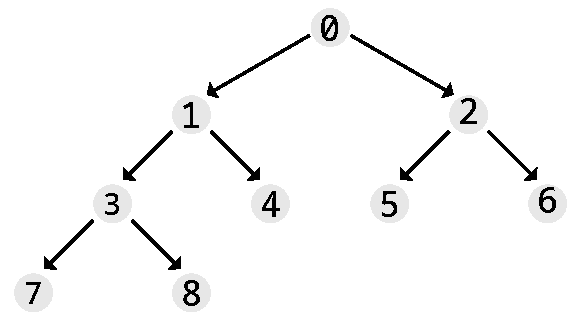
\includegraphics[scale=1]{figs/figure_heap.pdf}}
\caption{The heap corresponding to an array containing the digits 0 to 8}
\label{fig.heap}
\end{figure}

Here is one way to build a heap (in partial alphabetic order) 
from a list of unordered letters:

\begin{verbatim}
sub build-heap (@array, $index is copy) {
    my $index-val = @array[$index];
    while ($index) {
        my $parent = Int( ($index - 1) / 2);
        my $parent-val = @array[$parent];
        last if $parent-val lt $index-val;
        @array[$index] = $parent-val;
        $index = $parent;
    }
    @array[$index] = $index-val;
}

sub heapify (@array) {
    for @array.keys -> $i {
        build-heap @array, $i;
    }
}

my @input =  <m t f l s j p o b h v k n q g r i a d u e c>; 
heapify @input;
say @input;
\end{verbatim}

Note that the heap is built in place (there is no 
need for a second array). The resulting array is 
displayed as follows:
\begin{verbatim}
[a b g d c k j l f h e m n q p t r o i u s v]
\end{verbatim}

Is this a correct heap? It's difficult to say at first 
glance and checking it manually is somewhat tedious. When 
writing a program for building such a data structure, 
it is often useful to write some subroutines to display 
the content in a way that makes it easier to understand 
the result and check its correctness. The following 
code shows two examples of such possible subroutines:
\begin{verbatim}
sub print-heap (@array) {
    my $start = 0;
    my $end = 0;
    my $last = @array.end;
    my $step = 1;
    loop {
        say @array[$start..$end];
        last if $end == $last;
        $start += $step;
        $step *= 2;
        $end += $step;
        $end = $last if $end > $last;
    } 
}

sub print-heap2 (@array) {
    my $step = 0;
    for @array.keys -> $current {
        my $left_child = @array[2 * $current + 1];
        say "$current\tNode = @array[$current];\tNo child" 
             and next unless defined $left_child;
        my $right_child = @array[2 * $current + 2] // "' '";
        
        say "$current\tNode = @array[$current];\tChildren: " . 
             " $left_child and $right_child";
        $step++;
    }
}

\end{verbatim}

The first one displays the related tree level by level:

\begin{verbatim}
(a)
(b g)
(d c k j)
(l f h e m n q p)
(t r o i u s v)
\end{verbatim}

which makes it easy to draw the tree (see Figure~\ref{fig.heap2}).

\begin{figure}
\centerline
{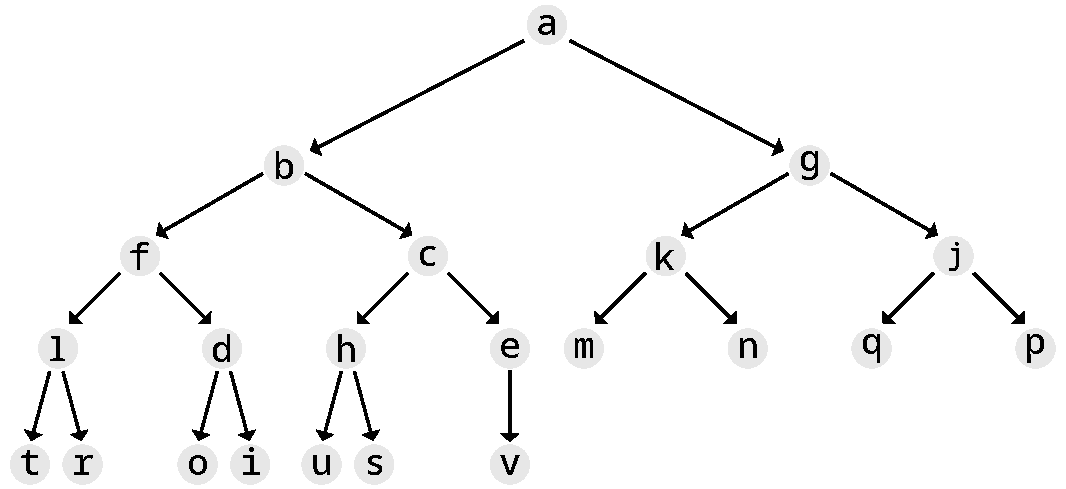
\includegraphics[scale=0.8]{figs/figure_heap2.pdf}}
\caption{The heap corresponding to the array of letters}
\label{fig.heap2}
\end{figure}


The second one shows the children for each node and makes it 
possible to easily check that the partial alphabetic order 
constraint is satisfied (i.e., each node is smaller than its 
children):

\begin{verbatim}
0       Node = a;       Children:  b and g
1       Node = b;       Children:  d and c
2       Node = g;       Children:  k and j
3       Node = d;       Children:  l and f
4       Node = c;       Children:  h and e
5       Node = k;       Children:  m and n
6       Node = j;       Children:  q and p
7       Node = l;       Children:  t and r
8       Node = f;       Children:  o and i
9       Node = h;       Children:  u and s
10      Node = e;       Children:  v and ' '
11      Node = m;       No child
12      Node = n;       No child
(...)
21      Node = v;       No child
\end{verbatim}



\section{Depuración de Programas}
\index{debugging}

Cuando depuras un programa, y especialmente si estás 
trabajando con un error bien difícil, aquí presentamos
algunas sugerencias que podrías intentar:

\begin{description}

\item[Reading] Examine your code, read it back to yourself, and
check that it says what you meant to say.

\item[Running] Experiment by making changes and running different
versions.  Often if you display the right thing at the right place
in the program, the problem becomes obvious, but sometimes you have to
build scaffolding.

\item[Running under a debugger] A {\bf debugger} is a utility 
program that enables you to run a program step by step, 
so you can follow the execution path and check the content of important 
variables at crucial points in the program execution, to set 
break points, etc. Perl~6 provides a debugger, called 
{\tt perl6-debug}, that makes all these things possible. With the 
advent of modern high-level languages, many people balk at 
using a debugger. This is a mistake. A debugger will not help 
solve every kind of problem, but it can be immensely 
useful. See Section~\ref{perl-debugger} for more information
on the Perl debugger.
\index{debugger}

\item[Ruminating] Take some time to think!  What kind of error
is it: syntax, runtime, or semantic?  What information can you get from
the error messages, or from the output of the program?  What kind of
error could cause the problem you're seeing?  What did you change
last, before the problem appeared?

\item[Rubber ducking] If you explain the problem to someone else, you
sometimes find the answer before you finish asking the question.
Often you don't need the other person; you could just talk to a rubber
duck.  That's the origin of the well-known strategy called {\bf
rubber duck debugging}.  I am not making this up; see 
\url{https://en.wikipedia.org/wiki/Rubber_duck_debugging}.
\index{rubber duck debugging}

\item[Retreating] At some point, the best thing to do is back
off, undoing recent changes, until you get back to a program that
works and that you understand.  Then you can start rebuilding.

\end{description}

Los programadores principiantes algunas veces se atascan en una de
estas actividades y se olvidan de las otras. Cada actividad viene
con su propio modo de fallo.
\index{typographical error}

Por ejemplo, leer tu programa podría ayudarte si el problema es
un error tipográfico, pero no si el problema es un malentendido 
conceptual. Si no entiendes lo que tu programa hace, puedes leerlo
más 100 veces y nunca verás el error, porque el problema se encuentras en
tu cabeza.
\index{experimental debugging}


Desarrollar experimentos puede ayudarte, especialmente si ejecutas
pruebas pequeñas y simples. Pero si desarrollas experimento sin pensar 
o leer tu código, puedes caer en un patrón que llamamos ``programación de 
paso aleatorio'', el cual es el proceso de hacer cambios aleatorios hasta
que el programa haga lo correcto. Obviamente, la programación de paso aleatorio
puede tomar mucho tiempo.
\index{random walk programming}
\index{development plan!random walk programming}

Debes tomar tiempo para pensar. La depuración es como un experimento científico.
Podrías tener por lo menos una hipótesis sobre el problema (por ejemplo, 
?`cuál es el problema?). Si hay más de dos posibilidades, intenta pensar
acerca de una prueba que eliminaría uno de ellos.

Aún así, la mejores técnicas de depuración fallarán si hay muchos errores,
o si el código que estás intentando arreglar es demasiado grande y 
complicado. Algunas veces la mejor opción es retroceder, simplificar el
programa hasta que obtengas algo que funcione y que entiendas.

Los programadores principiantes son usualmente reacios a retroceder
porque no pueden tolerar el hecho de borrar una línea de código 
(aún si es algo erróneo). Si te hace sentir mejor, haz una copia de
tu programa en otro archivo antes de hacer cambios. De esa manera
puedes copiar las piezas una a la vez con cada progreso.

Encontrar un error difícil requiere leer, ejecutar (sin o con 
un depurador), reflexionar, y algunas veces retroceder. Si te atasca
en una de estas actividades, prueba las otras. 


\section{Glosario}


\begin{description}

\item[Determinista] Perteneciente a un programa que hace la misma
cosa cada vez que se ejecuta, dado la misma entrada.
\index{deterministic}

\item[Pseudoaleatorio] Perteneciente a una secuencia de números que
aparece ser aleatoria, pero es generada por un programa determinista.
\index{pseudorandom}

\item[Valor por defecto] El valor dado a un parámetro opcional si 
no se provee un argumento.
\index{default value}

\item[Sobrescribir] Reemplazar un valor por defecto con un argumento.
\index{override}

\item[Benchmarking] El proceso de elegir entre varias estructuras de datos
y algoritmos al implementar alternativas y someterlas a pruebas (
especialmente sus tiempos de duración) con una muestra de las entradas
posibles
\index{benchmarking}

\item[Depurador] Un programa que permite ejecutar un programa línea
por línea y chequea su estado a cualquier paso durante su ejecución.
\index{debugger}

\item[Depuración del patito de goma] Depuración que involucra 
explicar tu problema a un objeto inanimado tal como un patito de goma.
Articular el problema puede ayudarte a solucionarlo, aún si el patito
de goma no sabe Perl.
\index{rubber duck debugging}
\index{debugging!rubber duck}

\end{description}

\section{Exercises: Huffman Coding}
\label{huffman_exercise}

Huffman coding is a technique used for data compression, i.e., 
to reduce the size of a piece of data (such as, for example, 
compressing a file).

\subsection{Variable-Length Codes}
\index{variable-length code}

If you are familiar with Morse code, you know that it is a 
system for encoding the letters of the alphabet as a series 
of dots and dashes. For example, the famous signal {\tt ...---...} 
represents the letters SOS, which comprise an 
internationally recognized call for help. The table 
in Figure~\ref{fig.morse} shows the rest of the codes.
\index{Morse code}

\begin{figure}
\centerline
{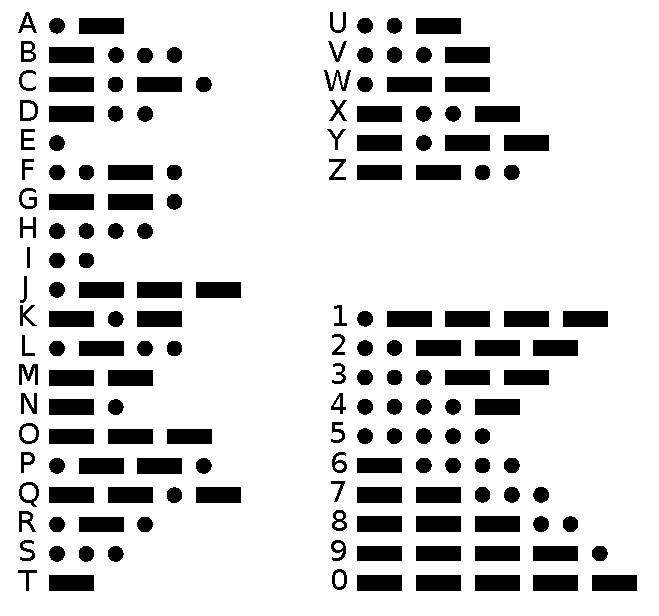
\includegraphics[scale=0.6]{figs/International_Morse_Code.pdf}}
\caption{International Morse code (public domain)}
\label{fig.morse}
\end{figure}

Morse code (invented between 1836 and 1844) was one of the 
very first attempts at digital encoding of the alphabet of a 
plain text. The only known earlier attempt is the braille 
alphabet (1824-1837).
\index{Morse, Samuel}
\index{braille alphabet}

Notice that some codes are longer than others. By design, the 
most common letters have the shortest codes. Since there are a 
limited number of short codes, that means that less common letters 
and symbols have longer codes. A typical message will have more 
short codes than long ones, which minimizes the average 
transmission time per letter.

Codes like this are called variable-length codes. In this exercise, 
we will look at an algorithm for generating a variable-length code 
called a Huffman code. It is an interesting algorithm in its own 
right, but it also makes a useful exercise because its implementation 
uses a variety of data structures.
\index{Huffman!code}

Here is an outline of what we will do until the end of this 
chapter:

\begin{enumerate}

\item First, we will use a sample of English text to generate 
a table of characters and their frequencies.

\item Then we will use this frequency table to generate a code 
table.

\item Finally, we will encode a message with this code table 
and then decode it.

\end{enumerate}

\subsection{The Frequency Table}
\index{frequency!table}

Since the goal is to give short codes to common letters, we 
have to know how often each letter occurs. In Edgar Allan Poe’s 
short story ``The Gold Bug,'' one of the characters, William~Legrand, 
uses letter frequencies to crack a cypher. He explains:
\index{Poe, Edgar Allan}
\index{The Gold-Bug (Edgar Allan Poe)}
\index{cypher}

\begin{quote}
``Now, in English, the letter which most frequently occurs 
is e. Afterwards, the succession runs thus: a o i d h n r s 
t u y c f g l m w b k p q x z. E however predominates so 
remarkably that an individual sentence of any length is 
rarely seen, in which it is not the prevailing character.''
\end{quote}

So our first mission is to see whether Poe got it right. 
To check, let's use as a sample the text of ``The Gold Bug'' 
itself, which can be downloaded from Project Gutenberg 
(\url{http://www.gutenberg.org/files/2147/2147-0.txt}) and 
a variety of other websites. 
\index{Project Gutenberg}

\begin{exercise}
\label{letter_frequency}
Write a program that counts the number of times each letter 
appears in a sample text. Download the text of ``The Gold Bug'' 
and analyze the frequency of the letters.

Solution: see Section~\ref{sol_letter_frequency}
\end{exercise}

\subsection{Building the Huffman Code}
\index{Huffman!code}

For our purposes, Morse code has one defect: it does not 
use just two symbols as you might think, but actually three: 
in addition to the dots and dashes, it it also implicitly 
using the space between two symbols, as well as a longer space 
between two letters.
\index{Morse code}

The reason why some space is needed is quite simple. Refer to the Morse 
code table above and suppose you receive three dots (\verb'...'). 
This could be interpreted as the letter ``e'' three times , or as 
``ie'' or ``ei,'' or as ``s'', or as the beginning of ``h,'' ``v,'' 
``3,'' ``4,'' or ``5''. Added spaces make it possible to disambiguate 
between those various possibilities. But they also make code 
transmission much slower.

In 1951, David A. Huffman invented a code-building technique avoiding 
this problem: provided that you know where a given letter starts, 
it is totally unambiguous. For example, we will meet later a Huffman 
code for a small subset of the alphabet that looks like this:
\index{Huffman, David A.}
\index{Huffman!code}

\begin{verbatim}
a => ..
e => .-
s => -.-
n => -..
t => --.
d => ---.
r => ----
\end{verbatim}

If you start reading a sequence of dots and dashes representing a 
valid text composed with these seven letters, you can always decode 
it without any ambiguity. If the first symbol is a dot, then the letter 
is either an ``a'' or a ``e'' depending on the next symbol. If the 
first symbol is a dash and the next one a dot, then the letter must 
be either a ``s'' or an ``n'' depending on the third symbol. If the 
two first symbols are dashes, you can similarly determine that the 
current letter is a ``t'' (if the third symbol is a dot), or a ``d'' 
or a ``r,'' which you can find out by looking at the fourth symbol. 
In brief, you don't need spaces between the symbols, it is always 
possible to unambiguously decode a letter.

How can we build such a Huffman code? Let's do it by hand with a 
very simple alphabet: the four letters of the nucleo-bases of DNA: A, 
C, T, and G. Suppose we want to encode the following input string:
\index{DNA (deoxyribonucleic acid)}
\index{alphabet}

\begin{verbatim}
CCTATCCTCGACTCCAGTCCA
\end{verbatim}

This gives the following frequency table:
\index{frequency!table}

\begin{verbatim}
C :     10      47.62
T :     5       23.81
A :     4       19.05
G :     2        9.52
\end{verbatim}

To build the Huffman code, we start with the two less frequent 
letters and merge them into one new temporary symbol, \verb"[GA]", 
which we pretend is a new composite letter with a 
frequency of 6. At this point, we decide that, between two letters, 
the less frequent one will have an appended dot and the other 
an appended dash (this is an arbitrary choice, it could be done 
the other way around). So we say that the symbol for the least 
common of the two letters (``G'') will be \verb'[GA].' and the 
symbol for ``A'' will be \verb'[GA]-'. 

We are now left with three letters, C, T, and [GA]. We merge the 
two least frequent letters, ``T'' and ``[GA],'' and can now tell 
that the symbol for ``T'' will be \verb'[TGA].' and the symbol for 
\verb'[GA]' will be \verb'[TGA]-'. There are only two letters left, 
``C'' and ``TGA``, with ``C'' the least frequent one; so ``C'' will 
be a dot and ``TGA`` a dash. 

We can now unroll our dummy letters: ``T'' is \verb'[TGA].', so, 
replacing \verb'[TGA]' with its symbol, i.e., a dash, the 
final code for ``T'' will be \verb'-.'; similarly, \verb'[GA].' 
now translates into \verb'--'. By the same substitution process, 
we can now determine that ``A'' is \verb'---' and ``G'' 
\verb'--.'. So our final Huffman code table is:
\index{Huffman!table}

\begin{verbatim}
C => .
T => -.
G => --.
A => ---
\end{verbatim}

Notice that, by construction, the most frequent letter (C) 
has the shortest code and the least common letters (G and A) 
the longest codes.

Manually encoding the \verb'CCTATCCTCGACTCCAGTCCA' input string 
with this code yields the following pseudo-Morse code:
\index{pseudo-Morse}

\begin{verbatim}
..-.----...-..--.---.-...-----.-...---
\end{verbatim}

Note that our Huffman code is not ambiguous: the first dot can 
only be a ``C,'' and the second one also. The next symbol is a 
dash, which can be the beginning of the three other letters, but 
only ``T'' can have a dot afterwards. The next sequence of 
symbols is four dashes; this can only be the three dashes of a 
``A'', with the last dash being the beginning of the next letter; 
and \verb'-.' can only be a ``T,'' and so on.
\index{Huffman!code}

In a real-life Huffman encoding for text file compression, 
we would not use dots and dashes, but 0 and 1 bits; however,  
dots and dashes are just another nice way of representing 
those binary values. So, let's just pretend that dots and dashes 
are really 0 and 1 binary numbers.
\index{binary number}
\index{bit}

\index{data compression}
Did we really achieve data compression? Our pseudo-Morse string has 
38~binary symbols. The original input string had 21 characters 
or bytes, that is 168 bits. The data has been compressed by a 
factor of about 4.4. 
\index{byte}

Is Huffman coding better than a fixed-length code? A string 
representation where each letter would be represented by two 
bits (two bits can represent four letters) would require 
42~symbols. So, yes, we did obtain a better data compression 
than a fixed-length encoding (by about 10\%). This may seem 
to be a small achievement, but this is actually quite good with 
such a small alphabet. With real text data, Huffman coding can 
achieve significant data compression.


\begin{exercise}
\label{huffman_code_2}
\begin{enumerate}
\item Write a program that performs Huffman encoding of a simple string 
of characters. You may start with the DNA example above. Don't 
worry, though, if you don't get the same Huffman table as the one 
above: there can be more than one Huffman code for a given input 
string; but check that you obtain an unambiguous code. 
\index{Huffman!code}
\item Try it with strings having a larger alphabet (you'll probably 
want to start with a relatively small alphabet, because it can 
otherwise be tedious to check the result by hand).
\item Write a subroutine to encode an input string into 
pseudo-Morse using the generated Huffman table.
\index{pseudo-Morse}
\index{alphabet}
\item Write a subroutine to decode the pseudo-Morse output 
you've just generated for the previous question.
\end{enumerate}
%
Solution: see Section~\ref{sol_huffman_code_2}.
\index{Huffman!code}
\end{exercise}

